\documentclass[12pt]{article}

\input preamble

\title{Principles of Parallel Architecture\\
Amdahl’s law and speed up}
\author{Xitong Liu \\
xliu@ece.udel.edu}

\begin{document}

\maketitle

\section{Serial Matrix Multiplication}
\begin{description}
\item[Requirement:] The first thing you need to do is to implement a C program 
for Matrix Multiplication, serially, for a single processor.

Your implementation will create and initialize 2 matrices of size N 
by N (that are called MatrixA and MatrixB) and multiply them (Store 
the result in a variable called MatrixC).

The value of N will be given to your program through the command line. 
The value of each element of the Matrices will be random double 
precision numbers from -1 to 1.

Also, for testing purposes, if N is less than 6, the program will 
automatically print to the screen matrices MatrixA, MatrixB and 
MatrixC.
\item[A:] 
Source Code:
\footnotesize
\begin{verbatim}
#include <stdio.h>
#include <stdlib.h>
#include <string.h>
#include <unistd.h>
#include <sys/time.h>

//global varialbes and definitions
#define OUTPUT_THRESHOLD 6

char * usage = "Usage: mm N\n";
char * matrix_size_error = "Invalid matrix size N = %d.
  It must be greater than 1.\n";
char * matrix_size_info = "Matrix Size N = %d\n";
char * malloc_error = "Malloc ERROR.\n";

void print_matrix(double * matrix, int matrixSize);

int main( int argc, char *argv[] )
{
  int matrixSize = 0;
  double * matrixA = NULL;
  double * matrixB = NULL;
  double * matrixC = NULL;
  
  struct timeval tv;
  struct timeval __start;
  struct timeval  __end;
  double t_start = 0.0f;
  double t_end = 0.0f;
  double Ti = 0.0f;
  double Tc = 0.0f;
  double Tt = 0.0f;

  int cycleI = 0;
  int cycleJ = 0;
  int cycleK = 0;

  if(argc < 2){
    puts(usage);
    exit(-1);
  }

  // get the matrix from the command line options list
  matrixSize = atoi(argv[1]);
  if(1 > matrixSize){
    printf(matrix_size_error, matrixSize);
    exit(-1);
  }
  printf(matrix_size_info, matrixSize);

  if(NULL == (matrixA = malloc( matrixSize * matrixSize * sizeof(double)))){
    puts(malloc_error);
    exit(-1);
  }
  if(NULL == (matrixB = malloc( matrixSize * matrixSize * sizeof(double)))){
    puts(malloc_error);
    free(matrixA);
    exit(-1);
  }
  if(NULL == (matrixC = malloc( matrixSize * matrixSize * sizeof(double)))){
    puts(malloc_error);
    free(matrixA);
    free(matrixB);
    exit(-1);
  }

  //initilize random generator
  gettimeofday(&tv, NULL);
  srand(tv.tv_sec * tv.tv_usec);
  gettimeofday(&__start, NULL);
  // initilize the matrix by random numbers between -1.00f and 1.00f
  for(cycleI = 0; cycleI < matrixSize * matrixSize; ++ cycleI){
    matrixA[cycleI] = (double)rand() / ((double)(RAND_MAX)+ 1.00) * 2.0 - 1.0;
    matrixB[cycleI] = (double)rand() / ((double)(RAND_MAX)+ 1.00) * 2.0 - 1.0;
  }
  gettimeofday(&__end, NULL);
  t_end = (__end.tv_sec + (__end.tv_usec/1000000.0));
  t_start = (__start.tv_sec + (__start.tv_usec/1000000.0));
  Ti = t_end - t_start;
  gettimeofday(&__start, NULL);
  // do the matrix multiplication
  for(cycleI = 0; cycleI < matrixSize; ++ cycleI){
    for(cycleJ = 0; cycleJ < matrixSize; ++ cycleJ){
      matrixC[cycleI * matrixSize + cycleJ] = 0.0f;
      for(cycleK = 0; cycleK < matrixSize; ++ cycleK){
        matrixC[cycleI * matrixSize + cycleJ] += 
          matrixA[cycleI * matrixSize + cycleK] *
          matrixB[cycleK * matrixSize + cycleJ];
      }
    }
  }
  gettimeofday(&__end, NULL);
  t_end = (__end.tv_sec + (__end.tv_usec/1000000.0));
  t_start = (__start.tv_sec + (__start.tv_usec/1000000.0));
  Tc = t_end - t_start;
  Tt = Ti + Tc;
  
  // if the matrix size is below the threshold, output the result
  if(matrixSize < OUTPUT_THRESHOLD){
    printf("MatrixA:\n");
    print_matrix(matrixA, matrixSize);
    printf("MatrixB:\n");
    print_matrix(matrixB, matrixSize);
    printf("MatrixC:\n");
    print_matrix(matrixC, matrixSize);
  }

  free(matrixA);
  free(matrixB);
  free(matrixC);
  printf("Ti: %fs\n", Ti);
  printf("Tc: %fs\n", Tc);
  printf("Tt: %fs\n", Tt);
  return 0;
}

void print_matrix(double * matrix, int matrixSize){
  int cycleI = 0;
  int cycleJ = 0;

  for(cycleI = 0; cycleI < matrixSize; ++ cycleI){
    for(cycleJ = 0; cycleJ < matrixSize; ++ cycleJ){
      if(matrix[cycleI * matrixSize + cycleJ] > 0.0f){
        printf("+%f\t", matrix[cycleI * matrixSize + cycleJ]);
      }else{
        printf("%f\t", matrix[cycleI * matrixSize + cycleJ]);
      }
    }
    printf("\n");
  }
}
\end{verbatim}
\end{description}

\section{Parallel Matrix Multiplication}
\begin{description}
\item[Requirement:]
In this case, you will use MPI to parallelize your Matrix 
Multiply application. As before, the names for the matrices 
will be MatrixA, MatrixB and MatrixC. Also, the size of the 
matrices remain NxN and N is a parameter passed through the 
command line.

The number of MPI processes to use is decided when the program 
is launched. For example if you run your program with:
\begin{verbatim}
mpirun �np 7 mpi_matmult 5 
\end{verbatim}
There will be 7 processors working to achieve the multiplication 
of 5x5 matrices. As before, when N is less than 6, automatically 
print the matrices to the screen.

\item[Q:] Create a directory called \texttt{mpi\_matmult}. Put in that directory all 
your source code files and the makefile that will correctly compile 
the program. Create a rule called �run� that will run the program with N=5

\item[Q:] Explain carefully how your program makes the parallel matrix 
multiplication and how your program satisfies the requirements a to f. 
Uses examples and mathematical analysis also.

\item[A:] I tried to distribute the matrix data evenly between the processes,
and each process initialize and calculate the data on it's own. More 
specifically, \texttt{MatrixA} and \texttt{MatrixC} were split into N parts
horizontally while \texttt{MatrixB} was split into N parts vertically,
say, \texttt{sub-MatrixA}, \texttt{sub-MatrixB}, \texttt{sub-MatrixC}.
Then in a loop of N, each processes used \texttt{MPI\_Bcast} to send 
it's part of \texttt{MatrixB} to other peers, calculated the multiplication
of \texttt{sub-MatrixA} and received \texttt{sub-MatrixB} and stored the 
result in \texttt{sub-MatrixC}. When the loop was done, each of the processes
have the result ready in \texttt{sub-MatrixC}. As last, process \#0 collected 
the results in a message ring through \texttt{MPI\_Send} and \texttt{MPI\_Recv}, 
validating the result by comparing with results from serial multiplication.

For each process, the total storage is roughly $\frac{4N^2}{P}$, holding 
\texttt{sub-MatrixA}, \texttt{sub-MatrixB}, \texttt{sub-MatrixC} and one 
intermediate sub-Matrix with the same size of \texttt{sub-MatrixB} to hold 
the data from other processes. Only process \#0 hold extra data to hold the 
collected data and do validation.

\item[Q:] How do you manage the distribution of the data when the sizes 
of your blocks are not multiple of the sizes of the matrix? For example 
when N=79 using 7 MPI processes.

\item[A:] To make sure the data is distributed evenly in the processes,
I made a division on the matrix size. For example, $79 = 7 \times 11 + 2$,
so each process will hold at least $11$ rows (columns) of data. For the 
remainder $2$, it will distributed evenly in the first $2$ processes. Thus,
$79 = 7 \times 11 + 2 = 2 \times 12 + 5 \times 11$. More specifically, 
process $\#0$ and $\#1$ will hold $12$ rows (columns) and others holding $11$
rows (columns).

\item[Q:] For the values of N that you found on part 1., measure the times 
$T_i$, $T_c$, and $T_T$ from 2 to the maximum of MPI processes supported.

Report your results in a graph of speed up vs number of MPI processes 
for each value of N used in part 1. All your plots have to be in the 
same graph. For the speed up uses $T_{t}$.

\item[A:] See Fig.\ref{fig: parallel_mm}. T0.5, T1, T480 etc,. denote the cases 
with different matrix size $N$ that the serial version will take 
different time span, i.e 0.5s, 1s, 480s (8 min), to get the result, respectively.
\begin{figure}[h!]
	\begin{center}
		\includegraphics[width=1.0\textwidth, angle=0]{parallel_mm.pdf}
		\caption{\label{fig: parallel_mm}Parallel Speedup $T_{T}$: Speedup vs Process Number}
	\end{center}
\end{figure}

\item[Q:] What is the best and the worst speed up? Why?
\item[A:] The best speed up is 42.1412 times when N = 10 and the original time is 
32s. The worst speed up is 4.0365 times when N = 2 and the original time is 240s 
(4 min).

The result is obvious: the more processes run concurrently, the higher speed up 
it will gain. 

For T0.5 case, the matrix size is very small (360 by 360). The speed
up decreases slowly as the process number increases. This is because the overhead to
start MPI and exchange data between processes is much longer than the time to run 
the multiplication and dominate the total time cost. The more process, the more overhead, 
and the speed up decreases as a result.

\item[Q: ] Repeat e. and f. using only $T_{C}$ for calculating the speed up.
\item[A: ] See Fig.\ref{fig: parallel_mm_2}. The result are similar with 
Fig.\ref{fig: parallel_mm} in which $T_{T}$ is measured. 

\begin{figure}[h!]
	\begin{center}
		\includegraphics[width=1.0\textwidth, angle=0]{parallel_mm_2.pdf}
		\caption{\label{fig: parallel_mm_2}Parallel Speedup $T_{C}$: Speedup vs Process Number}
	\end{center}
\end{figure}

The best speed up is 41.6632 times when N = 10 and the original time is 
32s. The worst speed up is 4.0502 times when N = 2 and the original time is 240s 
(4 min).

\item[Q: ] When is it a good idea to use parallel programming?
\item[A: ] When the data to be processed can be divided into non-overlap parts and can been 
processed separately, using parallel programming can gain great speed up.

\end{description}

\end{document}

\begin{comment}
\begin{figure}[h!]
	\begin{center}
		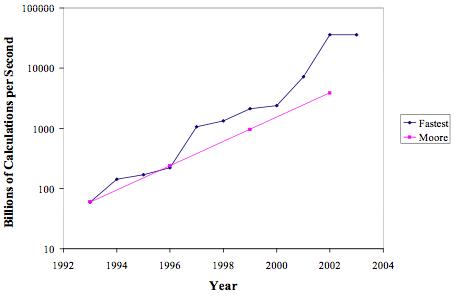
\includegraphics[width=0.7\textwidth, angle=0]{fatest.png}
		\caption{\label{fig:fatest}Fatest SuperComputer in the world}
	\end{center}
\end{figure}
\end{comment}